
\chapter{Uncomplicated Statistical \hnmr{} NMR Spectral Remodeling}

\section{Introduction}

\begin{doublespace}
{\bf FIXME}
\\\\
A second application of phase-scatter correction exists in the form of NMR
protein-ligand affinity screening. NMR spectroscopy reports a multitude of
time-averaged physical observables that carry information relating to the
nature of interactions between small molecule ligands and protein targets
\cite{lepre:chemrev2004}. A number of 1D \hnmr{} NMR pulse sequences have
been developed to probe these distinct features of binding, including
differences in free and bound ligand diffusion and relaxation properties
\cite{hajduk:jacs1997}, and saturation transfers from water
\cite{dalvit:jbnmr2000} and protein \cite{mayer:jacs2001} resonances. As part
of an NMR high-throughput screen, these 1D \hnmr{} NMR pulse sequences present
a number of unique challenges that include high false positive rates, long
acquisition times, and high demand for protein samples
\cite{lepre:menz2011,harner:jbnmr2013}. However, at suitably chosen
concentrations of ligand and protein, a standard, unedited 1D \hnmr{} NMR
experiment may be used to detect binding interactions through enhanced
relaxation rates of ligand spins
\cite{mercier:jacs2006,powers:ddt2008,mercier:cchts2009}.
\\\\
While it is possible to detect ligand binding using standard 1D \hnmr{} NMR,
the resulting spectra are a combination of free and bound ligand and protein
signals, a fact which makes them difficult to interpret. Broad, rolling
baselines arising from slowly tumbling protein spins are particularly
problematic during interpretation, as they often mask changes in ligand signal
broadness and intensity. This masking effect due to protein baselines is
exacerbated at protein-ligand concentration ratios nearing or exceeding unity,
forcing the use of excess ligand and increasing the false negative rate during
screening. To mitigate these issues, a statistical method called Uncomplicated
Statistical Spectral Remodeling (USSR), was developed that removes protein
baselines from high-throughput ligand-based screening datasets by leveraging
inter-sample reproducibility of protein signals. In addition, it will be
demonstrated that the use of phase-scatter correction greatly improves
inter-sample protein baseline reproducibility and reduces the false-positive
rate incurred by subsequent USSR-based analyses. The combination of PSC and
USSR enables a rapid analysis of standard 1D \hnmr{} NMR screening data,
especially in difficult cases having a high protein-ligand concentration ratio.
\end{doublespace}

\section{Materials and Methods}

\subsection{Sample Preparation and NMR Acquisition}

\begin{doublespace}
A set of 117 samples containing free ligand mixtures and a set of 117 samples
containing Bovine Serum Albumin (BSA) with ligand mixtures were prepared based
on previously published procedures \cite{powers:ddt2008,mercier:cchts2009}.
In summary, each mixture contained no more than four ligands, each ligand had
a concentration of 100 $\mu$M, and BSA had a concentration of 200 $\mu$M when
present. All NMR samples were prepared to 600 $\mu$L total volume in a buffer
containing 10 mM bis-tris-d$_{19}$, 1.0 mM NaCl, 1.0 mM KCl, 1.0 mM MgCl$_2$
and 10 $\mu$M trimethylsilyl propanoic acid (TMSP) in D$_2$O at pH 7.0
(uncorrected). Samples were loaded into standard 5 mm NMR tubes for spectral
acquisition.
\\\\
All NMR experiments were collected on a Bruker Avance DRX 500 MHz spectrometer
equipped with a 5 mm inverse triple-resonance (\hnmr{}, \cnmr{}, \nnmr{})
cryoprobe with a $z$-axis gradient. A Bruker BACS-120 sample changer and
ICON-NMR software were used to automate NMR data collection. Standard 1D
\hnmr{} NMR spectra were collected for each sample using a SOGGY water
suppression pulse sequence \cite{hwang:jmr1995,nguyen:jmr2007}. All
experiments were performed at 20 $^\circ$C with 256 scans, 8 dummy scans,
a carrier frequency offset of 2352.1 Hz, a 5482.5 Hz spectral width, and a 1.0
section inter-scan delay. Free induction decays were collected with 4$k$
complex data points, resulting in a total acquisition time of 8 minutes per
experiment.
\end{doublespace}

\subsection{NMR Data Processing}

\begin{doublespace}
Acquired NMR spectra were loaded and processed in batch inside the GNU Octave
3.6 programming environment \cite{eaton2008} using functions available in the
MVAPACK software package \cite{worley:acscb2014}. Free induction decays were
loaded in from Bruker DMX binary format and corrected for group delay by a
fixed circular shift. All decays were then zero-filled twice, Fourier
transformed and automatically phase corrected using a simplex optimization
routine. Phase-scatter correction was applied to a copy of the screen spectral
data, and spectral remodeling was performed in parallel on the uncorrected and
corrected datasets for the purposes of comparison.
\end{doublespace}

\begin{SCfigure}
\includegraphics[width=3.5in]{figs/ussr/01-baseline.png}
\caption
      [Statistical Baseline from the BSA Screening Dataset.]{
  {\bf Statistical Baseline from the BSA Screening Dataset.}
  \\
  Statistical baseline ($\boldsymbol{\mu} \pm 4 \boldsymbol{\sigma}$) computed
  from the \hnmr{} NMR ligand-based screen against BSA. The mean baseline is
  traced in deep red, while the confidence region for the baseline is filled
  in light red underneath.
}
\end{SCfigure}

\subsection{Statistical Spectral Remodeling}

\begin{doublespace}
The Uncomplicated Statistical Spectral Remodeling (USSR) method capitalizes on
the reproducibility of the protein baseline and the low likelihood that ligand
signals will dominate any given spectral data point across multiple samples.
For each pair of free mixture ($\mathbf{f}_n$) and screen (mixture plus
protein, $\mathbf{p}_n$) \hnmr{} NMR spectra, a difference spectrum
($\mathbf{d}_n$) was computed using a simple point-wise subtraction. The
central tendency ($\boldsymbol{\mu}$) and dispersion ($\boldsymbol{\sigma}$)
of the difference spectra were then robustly estimated using the median and
median absolute deviation, respectively. Figure 7.1 shows the statistical
baseline computed by USSR from a screen of ligand binding to BSA. Once a
statistical baseline is established for a given dataset, each spectrum
$\mathbf{p}_n$ in the screen is remodeled to maximally remove interference
from baseline signals. Each spectral data point in $\mathbf{p}_n$ is compared
to $\boldsymbol{\mu} \pm \boldsymbol{\sigma}$ using a Bonferroni-corrected
Student's $t$-test \cite{dunn:jasa1961}. The resulting $p$ value provides a
measure of how distinguishable the corresponding data point is from the
statistical baseline. Based on a preselected level of significance ($\alpha$),
data points having low $p$ values are retained (less the statistical baseline)
in the remodeled spectrum ($\mathbf{r}_n$) and data points having high $p$
values are modeled as Gaussian white noise. Figure 7.2 shows an example
remodeled spectrum from the ligand binding analysis of BSA.
\end{doublespace}

\begin{figure}[ht!]
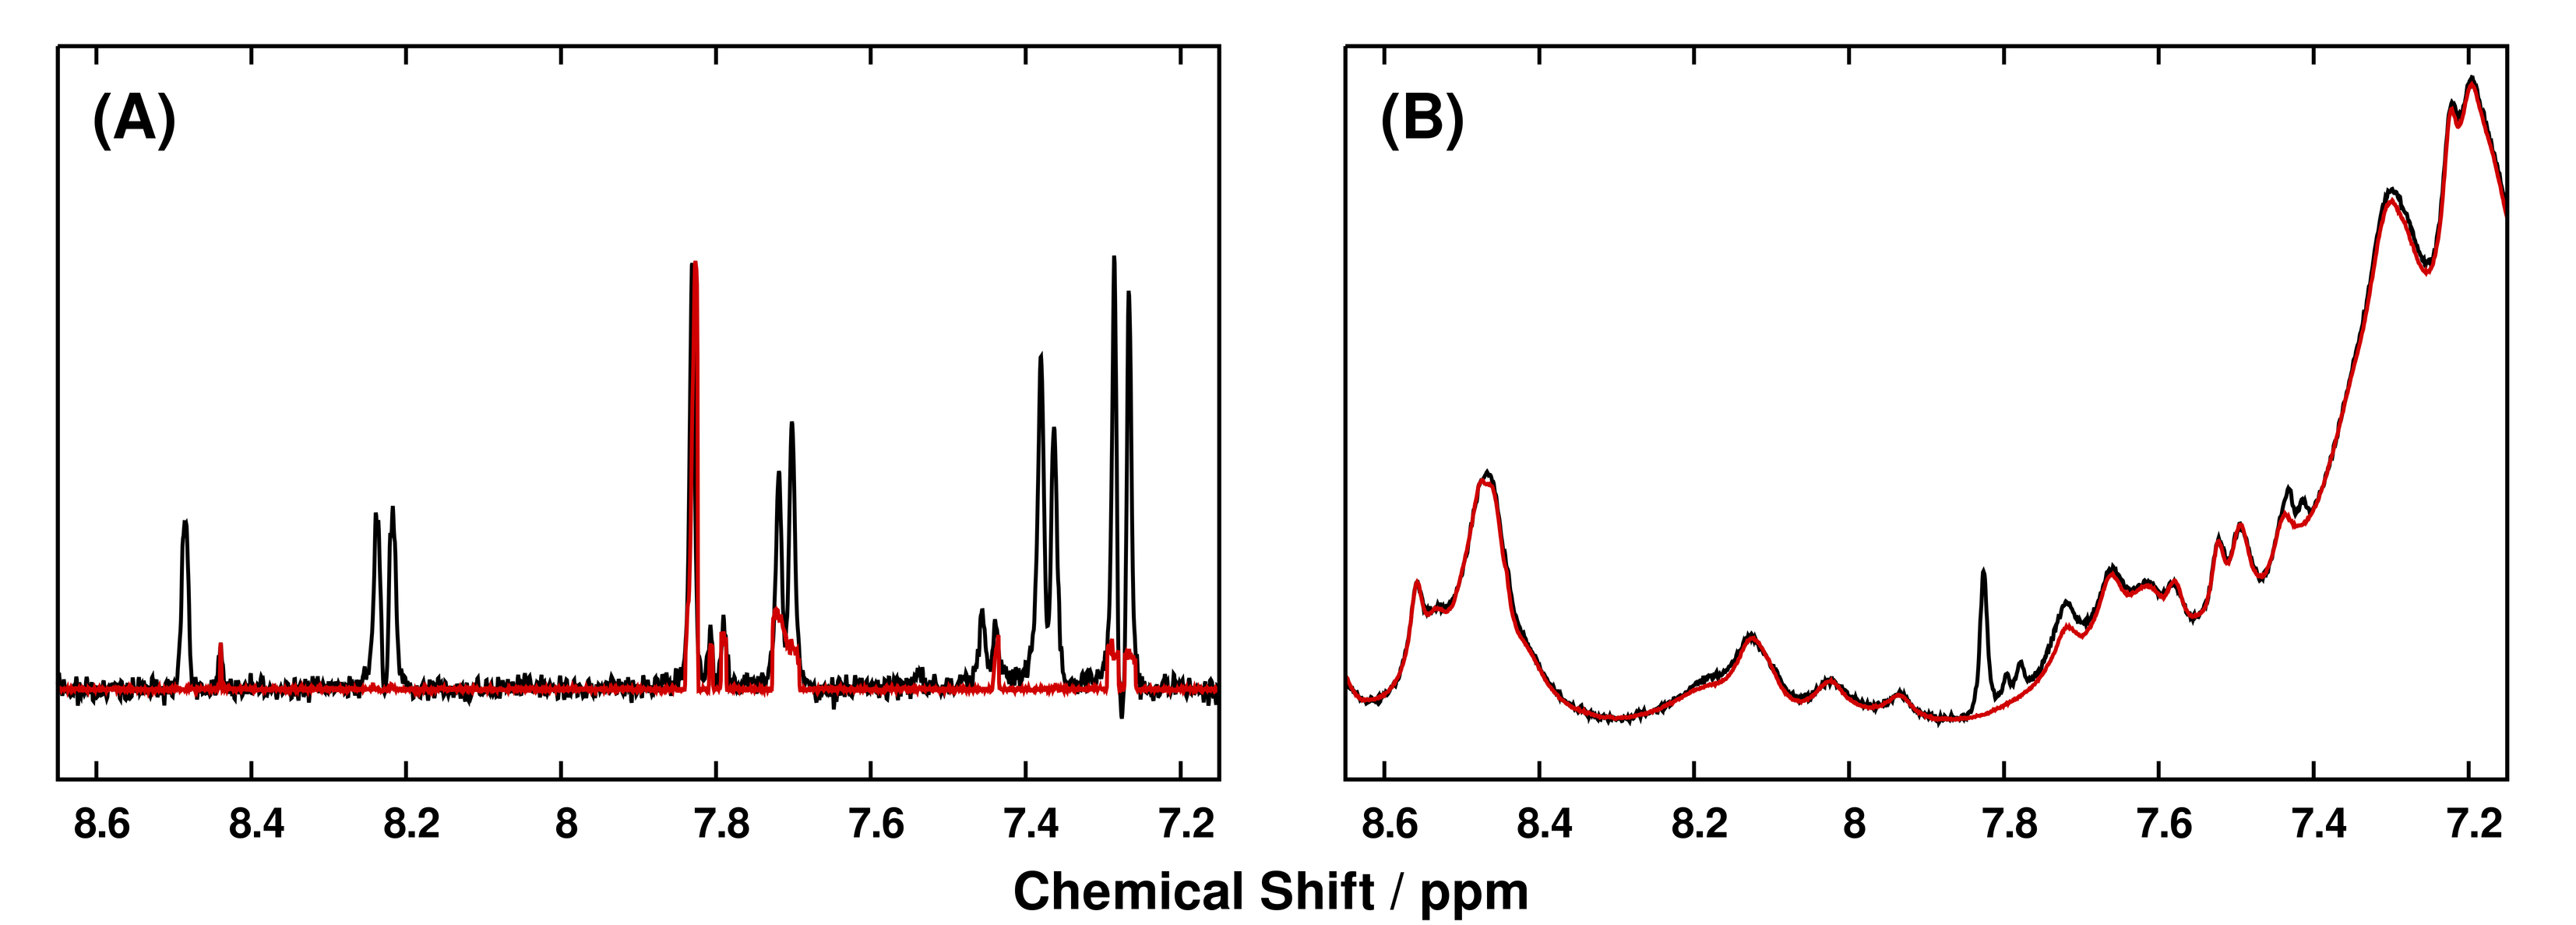
\includegraphics[width=6.5in]{figs/ussr/02-ussrfit.png}
\caption
      [Statistical Baseline Removal from a Screen Spectrum.]{
  {\bf Statistical Baseline Removal from a Screen Spectrum.}
  \\
  An example spectral remodeling result of tolazamide, dimethyl
  4-methoxyisophthalate, 1,7-dimethylxanthine and oxolinic acid in the
  presence of BSA, showing ({\bf A}) the free ligand spectrum (black) and
  the remodeled spectrum (red) resulting from removing the statistical
  baseline (red) from the screen spectrum (black) in ({\bf B}). The remodeled
  pseudospectrum readily indicates that several peaks from dimethyl
  4-methoxyisophthalate have broadened into the baseline due to interaction
  with BSA.
}
\end{figure}

\subsection{Statistical Hit Determination}

\begin{doublespace}
For each peak in each remodeled spectrum from USSR, a $K_D$ was computed based
on the intensity ratio between free and remodeled ligand signals. First, in the
limit of fast exchange between free and bound ligand states relative to the NMR
timescale, the fraction of bound ligand ($f_B$) was computed:
\begin{equation}
f_B =
 \left( \frac{I_F}{I_B} - 1 \right)
 \left( \frac{v_B}{v_F} - 1 \right)^{-1}
\end{equation}
where $I_F$ and $I_B$ are the intensities of free and remodeled (bound) ligand
signals, and $v_F$ and $v_B$ are the estimated NMR line widths of the free and
remodeled ligand signals, respectively \cite{shortridge:jcomb2008}. This
fast-exchange assumption may be safely regarded as valid in most
high-throughput 1D \hnmr{} NMR protein-ligand affinity screening experiments
\cite{lepre:chemrev2004}, where the width and intensity of each ligand signal
is a population-weighted sum of its values in the free and bound states.
Without any assumptions about relative concentrations of ligand and protein,
the fraction of bound ligand is related to the total protein concentration
$[P]_T$, total ligand concentration $[L]_T$ and $K_D$ via the following
equation \cite{shortridge:jcomb2008}:
\begin{equation}
f_B = \left[
  1 + \frac{2 K_D}{
    ([P]_T - [L]_T - K_D) + \sqrt{([P]_T - [L]_T - K_D)^2 + 4 K_D [P]_T}
  }
\right]^{-1}
\end{equation}

The solution of the above equation for $K_D$ yields the following result:
\begin{equation}
K_D = \frac{(f_B - 1)(f_B [L]_T - [P]_T)}{f_B}
\end{equation}
which was used to computed per-peak $K_D$ values for each remodeled spectrum
$\mathbf{r}_n$. Finally, the per-peak $K_D$ values were used to compute sample
mean and standard deviation $K_D$ values for each ligand. Hit detection was
accomplished by comparing per-ligand mean and standard deviation $K_D$ values
against a threshold via a Student's $t$-test, where a resulting $p$ value less
than a predefined significant $p$ value was reported as binding.
\end{doublespace}

\begin{figure}[ht!]
\includegraphics[width=6.5in]{figs/ussr/03-ussrfail.png}
\caption
      [Failed Baseline Removal due to Phase Errors.]{
  {\bf Failed Baseline Removal due to Phase Errors.}
  \\
  Example of a failed USSR result, highlighting the impact of phase error
  during computation and subtraction of the statistical baseline from a screen
  spectrum. Remodeled peaks ({\bf A}, red) upfield of 4.0 ppm are in fact not
  true signals, but were generated due to a phase-induced discrepancy between
  the statistical baseline ({\bf B}, red) and the screen spectrum
  ({\bf B}, black).
}
\end{figure}

\subsection{Analysis of Dataset Size}

\begin{doublespace}
A small simulation study was conducted to assess the quality of USSR
statistical baseline estimates over a range of sample sizes (number of spectral
pairs). For sizes from 2 to 116, the BSA dataset was randomly subsampled,
without replacement, to produce a smaller dataset. For each resultant dataset,
the statistical baseline was estimated, and its Pearson correlation to the true
statistical baseline was computed and stored. Over all numbers of spectral
pairs in the simulation, the median baseline correlations were computed, and
are reported in Figure 7.4.
\end{doublespace}

\begin{SCfigure}
\includegraphics[width=3.5in]{figs/ussr/04-blcorr.png}
\caption
      [Impact of Dataset Size on USSR Statistical Baselines.]{
  {\bf Impact of Dataset Size on USSR Statistical Baselines.}
  \\
  Correlation between statistical baselines from bootstrap-subsampled datasets
  of varying size and the original statistical baseline computed from the
  complete BSA dataset. Lines indicate median correlations, and shaded regions
  indicate confidence regions of plus or minus one standard deviation,
  estimated using median absolute deviation. Blue lines and shaded regions
  indicate values from subsampling the PSC normalized dataset, and red lines
  and shaded regions indicate values from subsampling the uncorrected dataset.
}
\end{SCfigure}

\section{Results}

\begin{doublespace}
FIXME.
\end{doublespace}

\section{Discussion}

\begin{doublespace}
FIXME.
\end{doublespace}

\section{Conclusions}

\begin{doublespace}
FIXME.
\end{doublespace}

\bibliographystyle{abbrv}
\bibliography{bworley}

